\documentclass[aspectratio=169]{beamer}
\usefonttheme{serif}
\usepackage{xeCJK}
\usepackage{fontspec}
\usepackage{graphicx}
\usepackage{listings}
\usepackage{xcolor}
\usepackage{indentfirst}
\usepackage{tikz}
\usepackage{amssymb}
\usepackage{amsthm}
\usepackage{amsmath}
\usepackage{tabularx}
\usepackage{hyperref}
\usepackage{ulem}
\usepackage{version}
\usepackage{thmtools}
\usepackage{qtree}
\usepackage{algpseudocode}
\usepackage{mathtools}
\usepackage{multicol}
\usepackage{xcolor}
\usepackage{animate}
\usepackage{graphicx}
\usepackage{svg}
\usepackage{media9}
\usepackage{subfigure}  
\usepackage{array}
\usepackage{longtable}
\usepackage[colorlinks,linkcolor=blue]{hyperref}
\usepackage{pgfplots}
\pgfplotsset{compat=newest}
\usepackage{pgfplotstable}
\usepackage{graphicx}
\usepackage[absolute,overlay]{textpos}

\AtBeginDocument{%
    \DeclareSymbolFont{pureletters}{T1}{\mathfamilydefault}{\mddefault}{it}%
    }

\XeTeXlinebreaklocale "zh"
\XeTeXlinebreakskip = 0pt plus 1pt

\usefonttheme{serif}
\usepackage[default]{opensans}
\setCJKmainfont{Noto Sans CJK TC}
\usetikzlibrary{arrows,decorations.markings,decorations.pathreplacing}
\newenvironment{Hint}{\noindent\textbf{Hint.}}{}

\tikzstyle {graph node} = [circle, draw, minimum width=1cm]
\tikzset{edge/.style = {decoration={markings,mark=at position 1 with %
            {\arrow[scale=2,>=stealth]{>}}},postaction={decorate}}}

\lstset{
    basicstyle=\ttfamily\normalsize,
    numberstyle=\normalsize,
    numbers=left,
    stepnumber=1,
    numbersep=3pt,
    commentstyle=\color{black!50},
    keywordstyle=\color{white!0!blue},
    stringstyle=\color{black!50!green},
    showspaces=false,
    showstringspaces=false,
    showtabs=false,
    tabsize=4,
    captionpos=b,
    breaklines=true,
    breakatwhitespace=false,
    escapeinside={\%*}{*)},
    morekeywords={*}
}

\AtBeginSection[]{
  \begin{frame}
  \vfill
  \centering
  \begin{beamercolorbox}[sep=8pt,center,shadow=true,rounded=true]{title}
    \usebeamerfont{title}\insertsectionhead\par%
  \end{beamercolorbox}
  \vfill
  \end{frame}
}


\title{HiPAC}
\author{NTHU-1}
\date{2024-08-08}

\usetheme{Madrid}
\usecolortheme{default}
\setbeamertemplate{itemize items}[square]
\setbeamertemplate{enumerate items}[default]
\setbeamertemplate{blocks}[default]

\begin{document}

    \begin{frame}
        \titlepage
    \end{frame}

    \section{Intro}
    \begin{frame}{隊伍名單 \& 分工}
        \begin{itemize}
            \item 陳奕嘉:Environment
            \item 蔡明妡:HPL, HPCG
            \item 許添睦、馬若晴:PIConGPU
            \item 陳克盈、李佳樺:NAMD
        \end{itemize}
    \end{frame}

    \section{Environment \& Benchmarks}
    \begin{frame}{Environment}
        \begin{block}{Network}
            \begin{itemize}
                \item MLNX\_OFED: Get access to InfiniBand
                \item IPoIB: IP over InfiniBand
                \item NFS: \texttt{/home} and \texttt{/opt} are shared between \texttt{pca1} and \texttt{pca2}
            \end{itemize}
        \end{block}
        \begin{block}{GPU}
            \begin{itemize}
                \item NVIDIA Drivers
                \item GPUDirect RDMA: Accelerate memory access
                \item CUDA \texttt{v11.8}, \texttt{v12.5}
                \item GDRCopy: Provides faster copy APIs for gpu memory
                \item NVIDIA HPC SDK
            \end{itemize}
        \end{block}
    \end{frame}
    
    \begin{frame}{Environment - GPU Direct RDMA}
        \begin{figure}
            \centering
            \includegraphics[width=1\linewidth]{rdma.png}
        \end{figure}
    \end{frame}
    
    \begin{frame}{Environment}
        \begin{block}{Module Management}
            \begin{itemize}
                \item Spack
                \item Lmod
            \end{itemize}
        \end{block}
        \begin{block}{Compilers}
            \begin{itemize}
                \item OneAPI \texttt{v2023.2}
                \item UCX \texttt{v1.17}
                \item OpenMPI \texttt{v4.1.6}, \texttt{v5.0.3} with CUDA and UCX
                \item MPICH \texttt{v4.2.2} with CUDA and UCX
            \end{itemize}
        \end{block}
    \end{frame}
    
    \begin{frame}{Environment}
        \begin{block}{Containers}
            \begin{itemize}
                \item Docker (integrated with NVIDIA Container)
                \item Singularity
                \item NVIDIA Container
            \end{itemize}
        \end{block}
    \end{frame}

    \begin{frame}{System Topo - CPU}
        \begin{itemize}
            \item CPU: Intel Gold 6154 $\times 2$ / node
            \item GPU: NVIDIA Tesla V100 SXM2 32GB  / node
            \item HPL: 46 TFlops
            \item HPCG: 2 TFlops
        \end{itemize}
        \begin{itemize}
            \item 2 NUMA node
            \begin{itemize}
                \item NUMA Node 0: CPU 0-17, GPU 0-3
                \item NUMA Node 1: CPU 18-35, GPU 4-7
            \end{itemize}
        \end{itemize}
    \end{frame}

    \begin{frame}{System Topo - GPU}
        \centering\includegraphics[width=0.9\textwidth]{nvidia-topo.png}
        \newline
        \texttt{nvidia-smi topo -m}
    \end{frame}

    \begin{frame}{System Topo - GPU}
        \centering\includegraphics[width=0.9\textwidth]{gputopo.png}
        \begin{itemize}
            \item green: NV1
            \item blue: NV2 (fastest)
        \end{itemize}
    \end{frame}

    \section{PIConGPU}        
        \begin{frame}{Build}
        \begin{block}{From Source}
            \begin{itemize}
            \begin{multicols}{2}
                \item GCC 11.4.0 
                \item CMAKE 3.29.2
                \item OpenMPI 4.1.4
                \item Boost 1.74.0
                \item openPMD 0.15.0 
                \item CUDA 12.5.82
                \item HDF5 1.12.1
            \end{multicols}
            \end{itemize}
        \end{block}
        \begin{block}{Container}
            \begin{itemize}
            \item Singularity \& NVIDIA Container.
            \item 不能更動 pmacc.
            \item 使用 PIConGPU 的 pmacc 但失敗.
            \end{itemize}
        \end{block}
        \end{frame}


        \begin{frame}{標準賽 - 結果}
        \begin{center}    
        \begin{tikzpicture}
            \begin{axis}[
                title={粒子數 - 總能量守恆誤差},
                xlabel={粒子數 (個)},
                ylabel={總能量守恆誤差 (‰)},
                grid=major,
                width=10cm,
                height=7cm,
            ]
            \addplot[
                color=blue,
                mark=o,
                ]
                coordinates {
                (192,3.628)
                (256,3.187)
                (320,2.777)
                (384,3.218)
                (512,3.437)
                };
            \end{axis}
        \end{tikzpicture}
        \end{center}
        \end{frame}
        
        \begin{frame}{標準賽 - 結果}
        \begin{center}    
        \begin{tikzpicture}
            \begin{axis}[
                title={網格大小 (X 倍的 debye length) - 總能量守恆誤差},
                xlabel={倍數 (倍)},
                ylabel={總能量守恆誤差 (‰)},
                grid=major,
                width=10cm,
                height=7cm,
            ]
            \addplot[
                color=blue,
                mark=o,
                ]
                coordinates {
                (1,3.187)
                (1.5,3.362)
                (2,2.777)
                (2.5,3.577)
                (2.95,3.031)
                };
            \end{axis}
        \end{tikzpicture}
        \end{center}
        \end{frame}

    \begin{frame}{標準賽 - 結果}
        \centering
        \includegraphics[width=0.40\textwidth]{dispersion.png}
        \newline
        \centering
        \texttt{steps 越高 -> 色散分析圖諧波效果越佳}
    \end{frame}


        \begin{frame}{時間步數 - Scalability}
            \begin{center}    
                \begin{tikzpicture}
                    \begin{axis}[
                        ybar,
                        symbolic x coords={1, 4, 16},
                        xtick=data,
                        ylabel={時間 (秒)},
                        ymin=4500,
                        ymax=5300,
                        bar width=15pt,
                        nodes near coords,
                        xlabel={GPU 數量},
                        enlarge x limits=0.2,
                        grid=both,
                        grid style={line width=.1pt, draw=gray!10},
                        major grid style={line width=.2pt,draw=gray!50}
                    ]
                        \addplot coordinates { (1, 5050.427) (4, 5152.49) (16, 5064.50)};
                    \end{axis}
                \end{tikzpicture}
            \end{center}
        \end{frame}
        
        \begin{frame}{平行賽 - Scalability}
            \begin{center}    
                \begin{tikzpicture}
                    \begin{axis}[
                        ybar,
                        symbolic x coords={4, 8, 16},
                        xtick=data,
                        ylabel={加速 (倍)},
                        ymin=0,
                        ymax=2,
                        bar width=15pt,
                        nodes near coords,
                        xlabel={GPU 數量},
                        enlarge x limits=0.2,
                        grid=both,
                        grid style={line width=.1pt, draw=gray!10},
                        major grid style={line width=.2pt,draw=gray!50}
                    ]
                        \addplot coordinates {(4, 1) (8, 1.61) (16, 1.67)};
                    \end{axis}
                \end{tikzpicture}
            \end{center}
        \end{frame}
        
        \begin{frame}{平行賽 - 結果}
            測試總 GPU 數量不變下,x, y 方向上不同數量的 GPU 組合對效能的影響
            \begin{table}
                \centering
                \begin{tabular}{c|c}
                    16 GPU 組合 (x * y) & 時間 (秒) \\ 
                    \hline
                    \texttt{16 * 1} & 950.9  \\
                    \texttt{8 * 2} & 952.3  \\
                    \texttt{4 * 4} & 953.4  \\
                    \texttt{2 * 8} & 957.5  \\
                \end{tabular}
            \end{table}
            \begin{table}
                \centering
                \begin{tabular}{c|c}
                    8 GPU 組合 (x * y) & 時間 (秒) \\ 
                    \hline
                    \texttt{8 * 1} & 988.6  \\
                    \texttt{4 * 2} & 1012.5  \\
                    \texttt{2 * 4} & 1002.2  \\
                \end{tabular}
            \end{table}
        \end{frame}
        
        \begin{frame}{平行賽 - Out of graphic memory}
            \begin{itemize}
                \item 當 GPU 低於四個的時候會發生 
                \newline
                \item 把 x 方向的網格數量除以二後,就能使用兩個 GPU 執行
                \newline
                \item 推測 PIConGPU 運用顯存的原理
            \end{itemize}
        \end{frame}
                   
        \begin{frame}{總 GPU 時間}
            \centering
            \begin{Large}
                539,000 秒
                \newline
                \newline
            \end{Large}

            \centering
            \begin{Huge}
                6.24 天
            \end{Huge}
        \end{frame}

    \section{NAMD}
    
    \begin{frame}{NAMD}
        \begin{block}{CASE01}
            約五萬顆原子的胰島素蛋白系統。 \\
            需要分別優化使用單節點純 CPU 平行和單節點 CPU + GPU 平行的性能。
        \end{block}

        \begin{block}{CASE02}
            200 組約六百顆原子的類蛋白澱粉系統。 \\
            每筆測資只能使用單節點平行,須最佳化整體測資時間。
        \end{block}

        \begin{block}{CASE03}
            一千萬顆原子的病毒蛋白系統。\\
            最佳化跨節點性能。
        \end{block}
    \end{frame}

    \begin{frame}{執行版本}
        \begin{itemize}
            \item multicore (for case01)
            \item multicore-CUDA (for case01 \& case02)
            \item verbs-smp-CUDA (for case03)
            \item gcc-verbs-linux-x86\_64-smp (build from source, for case03)
        \end{itemize}
    \end{frame}

    \begin{frame}{Build From Source}
        \begin{block}{Compilers}
            \begin{itemize}
                \item GCC: gcc 11.4.0
                \item MPI: OpenMPI 4.1.6
                \item CUDA: CUDA 11.8.0
            \end{itemize}
        \end{block}
        \begin{block}{Options}
            \begin{itemize}
                \item with \texttt{-O3}
                \item Infiniband version
                \item enable smp option
                \item use FFTW3
            \end{itemize}
        \end{block}
    \end{frame}
    
    \begin{frame}{CASE01 CPU Only - CORENUM Tuning}
        \begin{center}    
        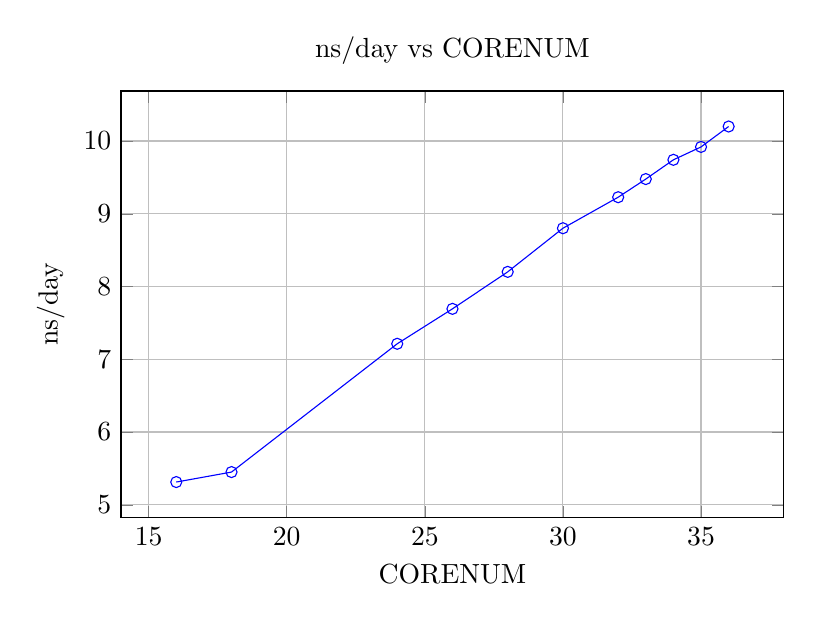
\begin{tikzpicture}
            \begin{axis}[
                title={ns/day vs CORENUM},
                xlabel={CORENUM},
                ylabel={ns/day},
                grid=major,
                width=10cm,
                height=7cm,
            ]
            \addplot[
                color=blue,
                mark=o,
                ]
                coordinates {
                (16,5.31236719)
                (18,5.44959128)
                (24,7.2131857)
                (26,7.69325455)
                (28,8.20162884)
                (30,8.80134485)
                (32,9.22781633)
                (33,9.47723568)
                (34,9.74193611)
                (35,9.91896208)
                (36,10.1996999)
                };
            \end{axis}
        \end{tikzpicture}
        \end{center}
    \end{frame}

    \begin{frame}{CASE01 CPU Only - CORENUM Tuning}
        \begin{center}
        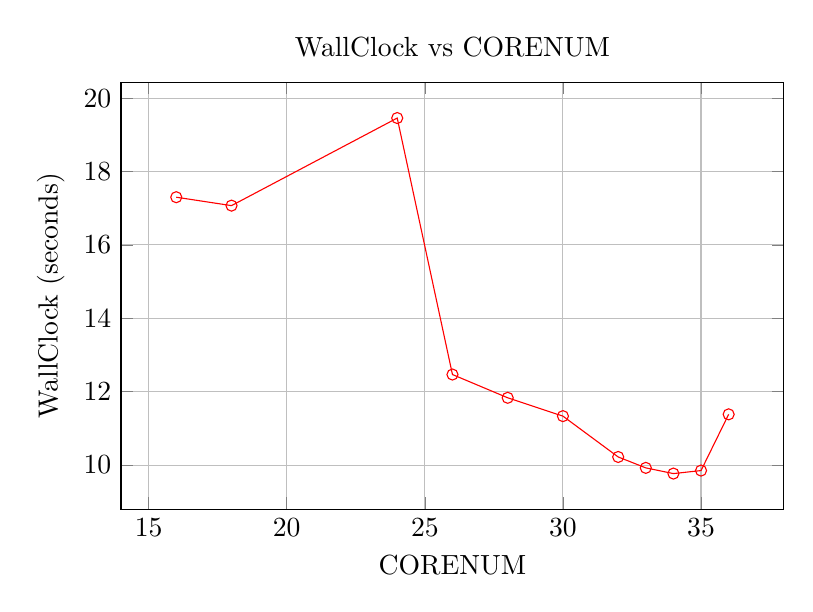
\begin{tikzpicture}
            \begin{axis}[
                title={WallClock vs CORENUM},
                xlabel={CORENUM},
                ylabel={WallClock (seconds)},
                grid=major,
                width=10cm,
                height=7cm,
            ]
            \addplot[
                color=red,
                mark=o,
                ]
                coordinates {
                (16,17.299942)
                (18,17.070303)
                (24,19.457312)
                (26,12.466978)
                (28,11.832924)
                (30,11.333097)
                (32,10.220497)
                (33,9.923141)
                (34,9.767454)
                (35,9.849663)
                (36,11.382466)
                };
            \end{axis}
        \end{tikzpicture}
        \end{center}
    \end{frame}

    \begin{frame}{CASE01 CPU+GPU - GPUNUM Tuning}
        set CORENUM=24 \\
        \begin{center}
        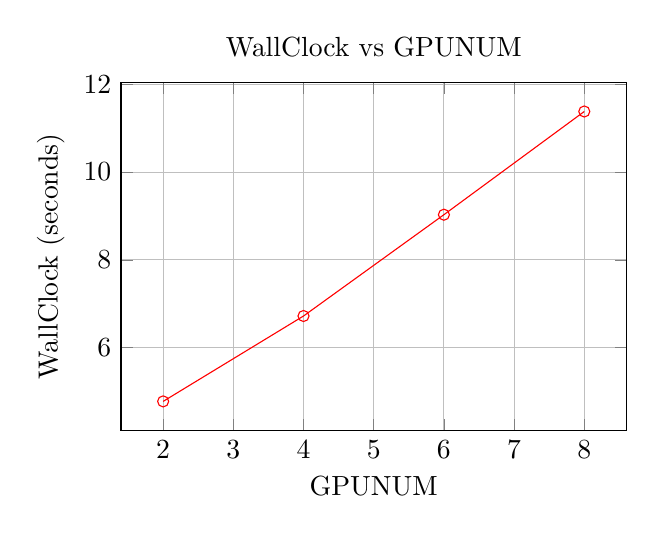
\begin{tikzpicture}
            \begin{axis}[
                title={WallClock vs GPUNUM},
                xlabel={GPUNUM},
                ylabel={WallClock (seconds)},
                grid=major,
                width=8cm,
                height=6cm,
            ]
            \addplot[
                color=red,
                mark=o,
                ]
                coordinates {
                (2,4.778053)
                (4,6.72243)
                (6,9.029081)
                (8,11.379419)
                };
            \end{axis}
        \end{tikzpicture}
        \end{center}
    \end{frame}

    
    \begin{frame}{CASE01 CPU+GPU - GPUNUM Tuning}
        set CORENUM=24 \\
        \begin{center}
        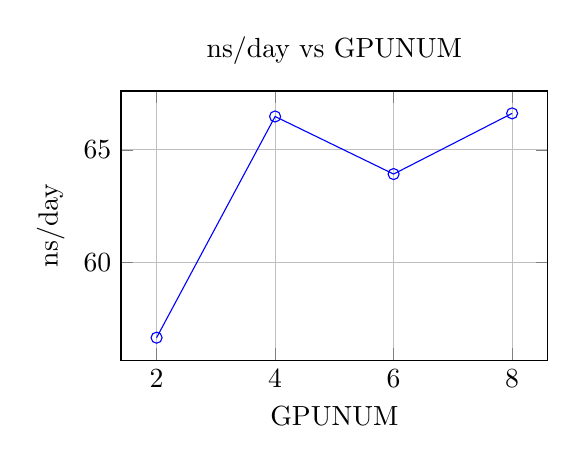
\begin{tikzpicture}
            \begin{axis}[
                title={ns/day vs GPUNUM},
                xlabel={GPUNUM},
                ylabel={ns/day},
                grid=major,
                width=7cm,
                height=5cm,
            ]
            \addplot[
                color=blue,
                mark=o,
                ]
                coordinates {
                (2,56.679703)
                (4,66.4747761)
                (6,63.9251309)
                (8,66.6120448)
                };
            \end{axis}
        \end{tikzpicture}
        \end{center} \\
        在 GPUNUM 為 2 時, WallClock 最低 ns/day 也最低,而 GPUNUM 為 4 ~ 8 時 WallClock 最高而 ns/day 也較為理想。
    \end{frame}

    \begin{frame}{CASE01 CPU+GPU - Minimizing WallClock}
        set DEVICE=0,1 \\
        \begin{center}
        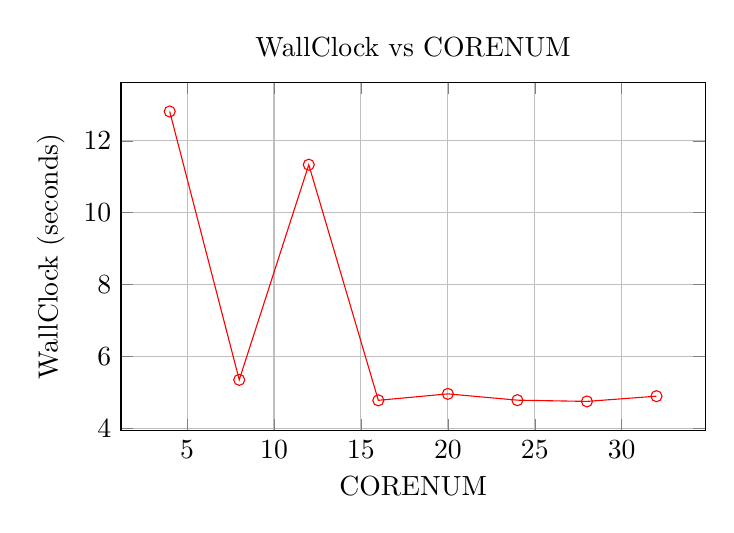
\begin{tikzpicture}
            \begin{axis}[
                title={WallClock vs CORENUM},
                xlabel={CORENUM},
                ylabel={WallClock (seconds)},
                grid=major,
                width=9cm,
                height=6cm,
            ]
            \addplot[
                color=red,
                mark=o,
                ]
                coordinates {
                (4,12.818184)
                (8,5.344539)
                (12,11.335964)
                (16,4.774245)
                (20,4.953531)
                (24,4.778053)
                (28,4.743882)
                (32,4.889291)
                };
            \end{axis}
        \end{tikzpicture}
        \end{center}
    \end{frame}

    \begin{frame}{CASE01 CPU+GPU - Maximize ns per day}
        \begin{center}
        \begin{longtable}{|c|c|c|}
        \hline
        \textbf{CORENUM} & \textbf{DEVICE} & \textbf{ns/day} \\
        \hline
        32 & 0,1,2,3 & 79.0964027 \\
        \hline
        35 & 0,1,2,3,4,5,6 & 81.143803 \\
        \hline
        32 & 0,1,2,3,4,5,6,7 & 78.9895655 \\
        \hline
        36 & 0,1,2,3,4,5,6,7 & 78.4553707 \\
        \hline
        \end{longtable}
        \end{center} 
    \end{frame}
    
    \begin{frame}{CASE02 multiple small cases - Try different CPU/GPU sets}
        \begin{longtable}{|c|c|c|}
        \hline
        \textbf{CORENUM} & \textbf{DEVICE} & \textbf{Total Time} \\
        \hline
        12 & 0,1 & 40m30s \\
        \hline
        16 & 0,1 & 15m56s \\
        \hline
        8 & 0,1,2,3 & 47m6s \\
        \hline
        16 & 0,1,2,3 & 46m13s \\
        \hline
        16 & 0,1,2,3,4,5,6,7 & 1h1m16s \\
        \hline
        \end{longtable}
        因為每筆測資規模很小,所以用太多 CORE 會沒辦法順利平行,\\
        而用太多 GPU 則會導致前置作業過久,執行時間太長。
    \end{frame}

    
    \begin{frame}{CASE02 multiple small cases - Optimize run scripts}
        但仔細觀察 run.bash 後我們發現...
        \begin{figure}
            \centering
            \includegraphics[width=0.4\linewidth]{case02_1.png}
            \label{fig:enter-label}
        \end{figure}
    \end{frame}

    
    \begin{frame}{CASE02 multiple small cases - Optimize run scripts}
        透過修改 scripts 來平行化測資以及透過 numactl 來指定每個測資執行時所使用的核心,而 namd2 本身也可以指定執行時所使用的 gpu。 \\
        實現了影分身之術!
        \begin{figure}
            \centering
            \includegraphics[width=0.65\linewidth]{case02_2.png}
            \label{fig:enter-label}
        \end{figure}
    \end{frame}
    
    \begin{frame}{CASE02 multiple small cases - Optimize run scripts}
        \begin{longtable}{|c|c|c|}
        \hline
        \textbf{CORENUM} & \textbf{DEVICE} & \textbf{Total Time} \\
        \hline
        0-15 + 16-31 & 0,1 + 2,3 & 10m16s \\
        \hline
        0-11 + 12-23 + 24-35 & 0,3 + 1,2 + 4,7 & 7m56s \\
        \hline
        \multicolumn{2}{|c|}{前4張 GPU 1:5, 後4張 GPU 1:4} & 3m7s \\
        \hline
        \multicolumn{2}{|c|}{前8張 GPU 1:5, 後8張 GPU 1:4} & 1m54s \\
        \hline
        \end{longtable}
    \end{frame}

    \begin{frame}{CASE03 large system - Minimize WallClock}
        \begin{center}
        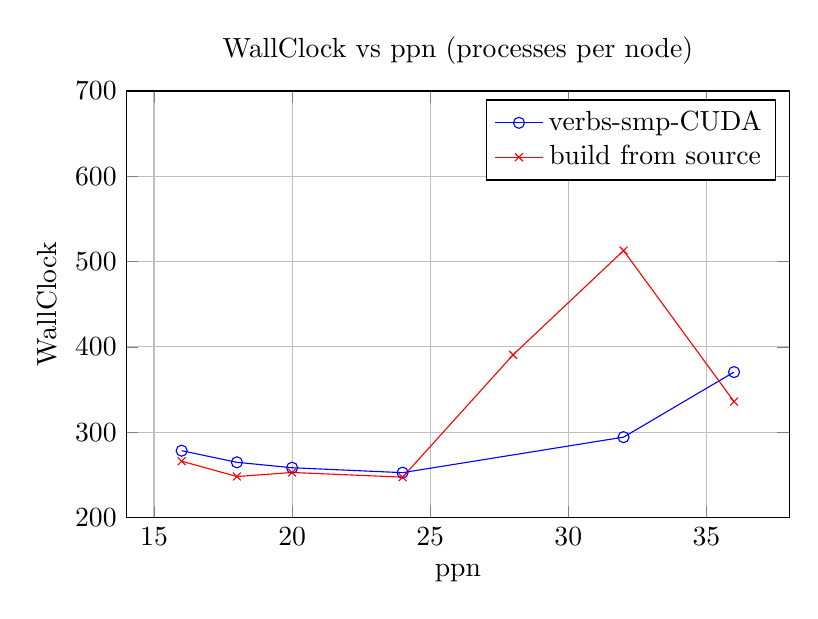
\begin{tikzpicture}
            \begin{axis}[
                title={WallClock vs ppn (processes per node)},
                xlabel={ppn},
                ylabel={WallClock},
                ymin=200,
                ymax=700,
                grid=major,
                width=10cm,
                height=7cm,
            ]
            \addplot[
                color=blue,
                mark=o,
                ]
                coordinates {
                (16,278.398468)
                (18,264.791016)
                (20,258.438812)
                (24,252.664856)
                (32,294.279358)
                (36,370.56076)
                };
                
            \addplot[
                color=red,
                mark=x,
                ]
                coordinates {
                (16,266.106659)
                (18,248.123840)
                (20,252.879349)
                (24,247.400513)
                (28,390.733032)
                (32,512.941467)
                (36,335.945862)
                };
                
            \legend{verbs-smp-CUDA, build from source}
            \end{axis}
        \end{tikzpicture}
        \end{center}
    \end{frame}


    \begin{frame}{CASE03 large system - Maximize ns per day}
        \begin{center}
        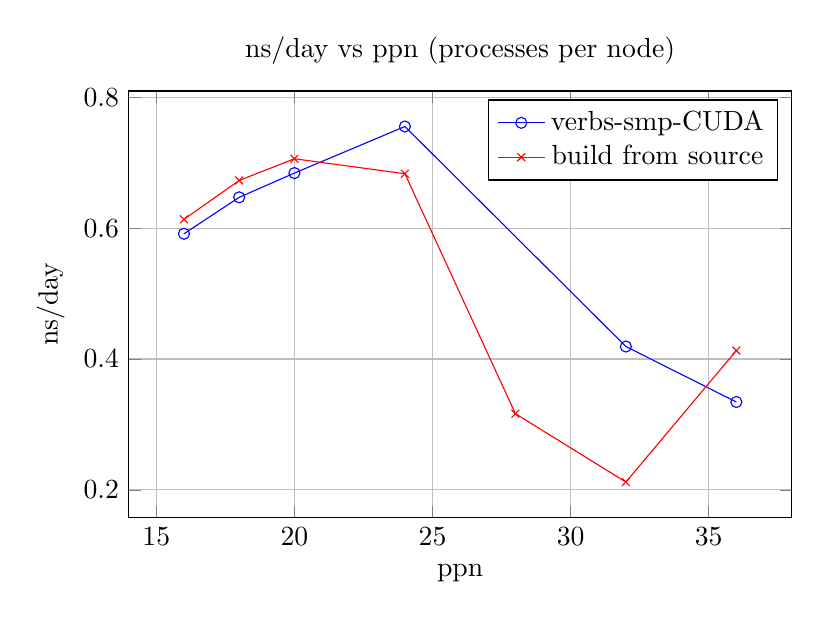
\begin{tikzpicture}
            \begin{axis}[
                title={ns/day vs ppn (processes per node)},
                xlabel={ppn},
                ylabel={ns/day},
                grid=major,
                width=10cm,
                height=7cm,
            ]
            \addplot[
                color=blue,
                mark=o,
                ]
                coordinates {
                    (16,0.5914884)
                    (18,0.6472491)
                    (20,0.68431749)
                    (24,0.755509553)
                    (32,0.419151888)
                    (36,0.334339696)
                };
                
            \addplot[
                color=red,
                mark=x,
                ]
                coordinates {
                    (16,0.61352328)
                    (18,0.673019975)
                    (20,0.70619474)
                    (24,0.683251457)
                    (28,0.316447685)
                    (32,0.211918733)
                    (36,0.412931358)
                };
                
            \legend{verbs-smp-CUDA, build from source}
            \end{axis}
        \end{tikzpicture}
        \end{center}
    \end{frame}

    \section{隱藏題}

    \begin{frame}{Hash 解密}
        \begin{itemize}
            \item URL: 根據後綴等號判斷出是 base64 編碼
            \item Tool: HashCat \texttt{v6.2.6}
            \item \texttt{hint.txt}: 使用掩碼攻擊成功破解
        \end{itemize}
        \begin{alertblock}{遇到的問題}
            \begin{itemize}
                \item \texttt{-a} 選項設定錯誤
                \item 自訂字典集時執行錯誤,疑似字典集過小
            \end{itemize}
        \end{alertblock}
        \begin{block}{解決辦法}
            \begin{itemize}
                \item 正確設定暴力攻擊模式
                \item 不使用字典集
                \item 可能方法:合併多種字典集
            \end{itemize}
        \end{block}
    \end{frame}

    \begin{frame}{PyFR}
        \begin{itemize}
            \item 流體力學軟體
            \item 照著官網安裝 dependency (apt, pip)
            \item metis 套件有問題,造成無法分割資料
            \item 進而導致無法執行
        \end{itemize}
    \end{frame}

    \section{其他}

    \begin{frame}{時間分配 \& 策略}
        \begin{itemize}
            \item Day 1:
            \begin{itemize}
                \item 裝機、研究測資
                \item 編譯所需 lib, bin
                \item 測試執行、排定晚間執行腳本
            \end{itemize}
            \item Day 2:
            \begin{itemize}
                \item 統整前一天執行結果
                \item 利用得到的最佳參數執行不同的版本
            \end{itemize}
            \item Day 3:
            \begin{itemize}
                \item 整理最佳結果、製作簡報
                \item 研究隱藏題
            \end{itemize}
        \end{itemize}
    \end{frame}

\end{document}